\documentclass[english]{article}
\usepackage[usenames,dvipsnames,svgnames,table]{xcolor}
\usepackage{babel,blindtext}
\usepackage{graphicx}
\usepackage{caption}
\usepackage{subcaption}
\usepackage{tabularx}
\usepackage{amsmath}
\usepackage{mathrsfs}
\usepackage{setspace}
\usepackage{enumerate}
\usepackage{todonotes}
\usepackage{listings}
\usepackage{paralist}
\usepackage{natbib}
\usepackage{fullpage}
\usepackage[T1]{fontenc}
\usepackage{booktabs}
\usepackage{pgfplotstable}
\usepackage{makecell}
\usepackage{comment}

\usepackage[colorlinks=true,
            linkcolor=blue,
            urlcolor=blue,
            citecolor=blue,
            final,
            hypertexnames=false]{hyperref}

%
%
%
\title{\bf{SoV Scaling Study}}
\author{Nicholas Malaya, Robert D. Moser \\ Institute for Computational Engineering and Sciences \\ University of Texas at Austin} \date{}

\begin{document}
\maketitle

Here, we investigate the variation of the Solar Vortex (SoV) as a function of diameter of the apparatus. 

\begin{figure}[!htb]
\minipage{0.32\textwidth}
  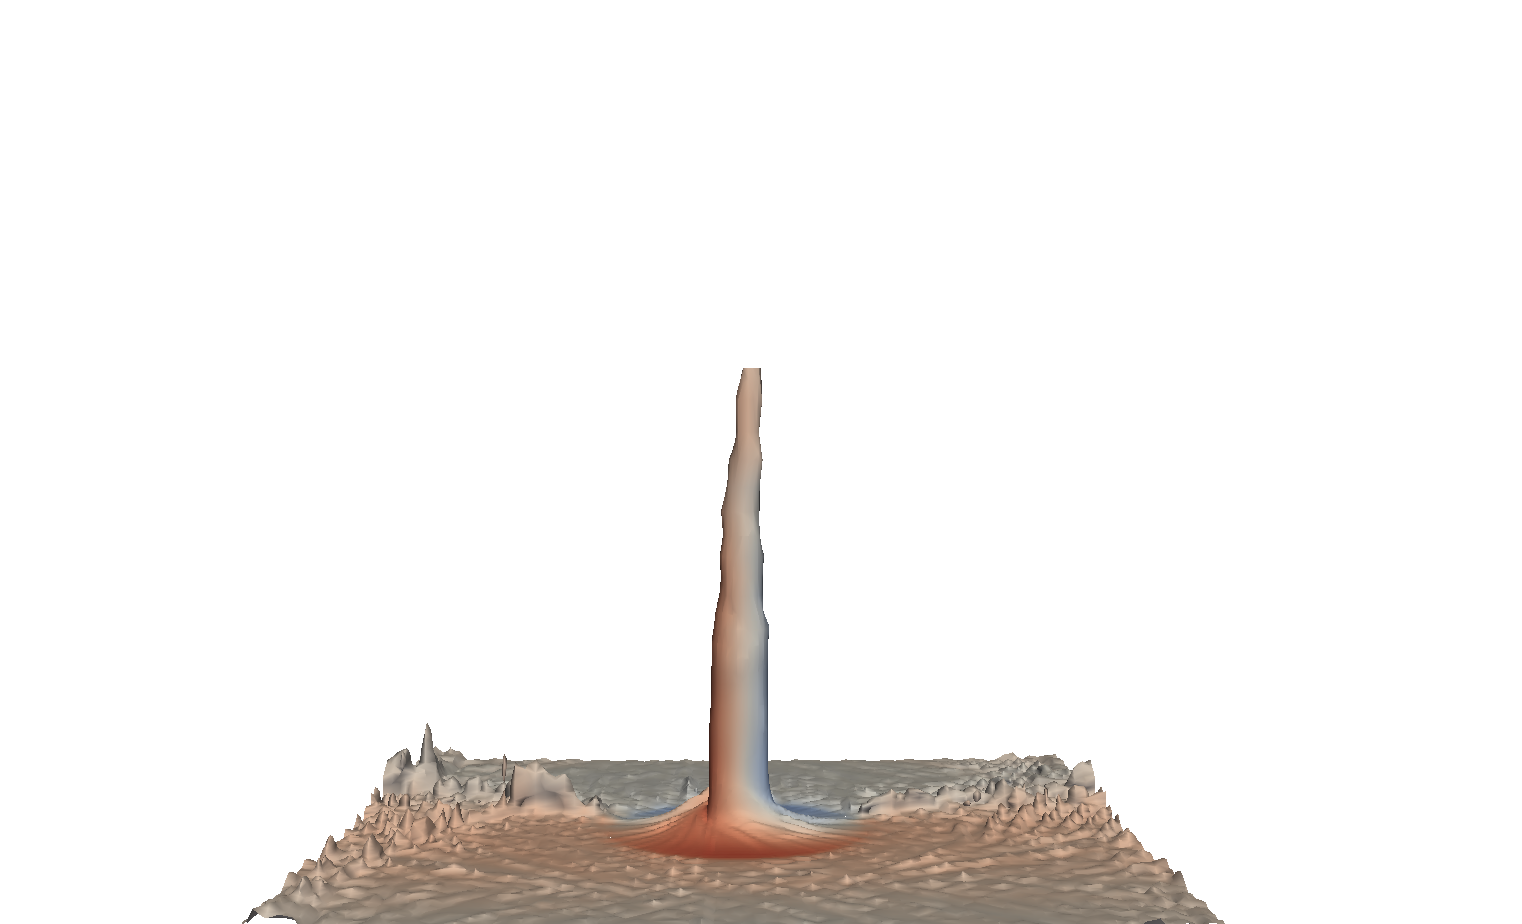
\includegraphics[width=\linewidth]{figs/1m_temp_iso}
  \caption{1m Apparatus}\label{fig:1m_scaling}
\endminipage\hfill
\minipage{0.32\textwidth}
  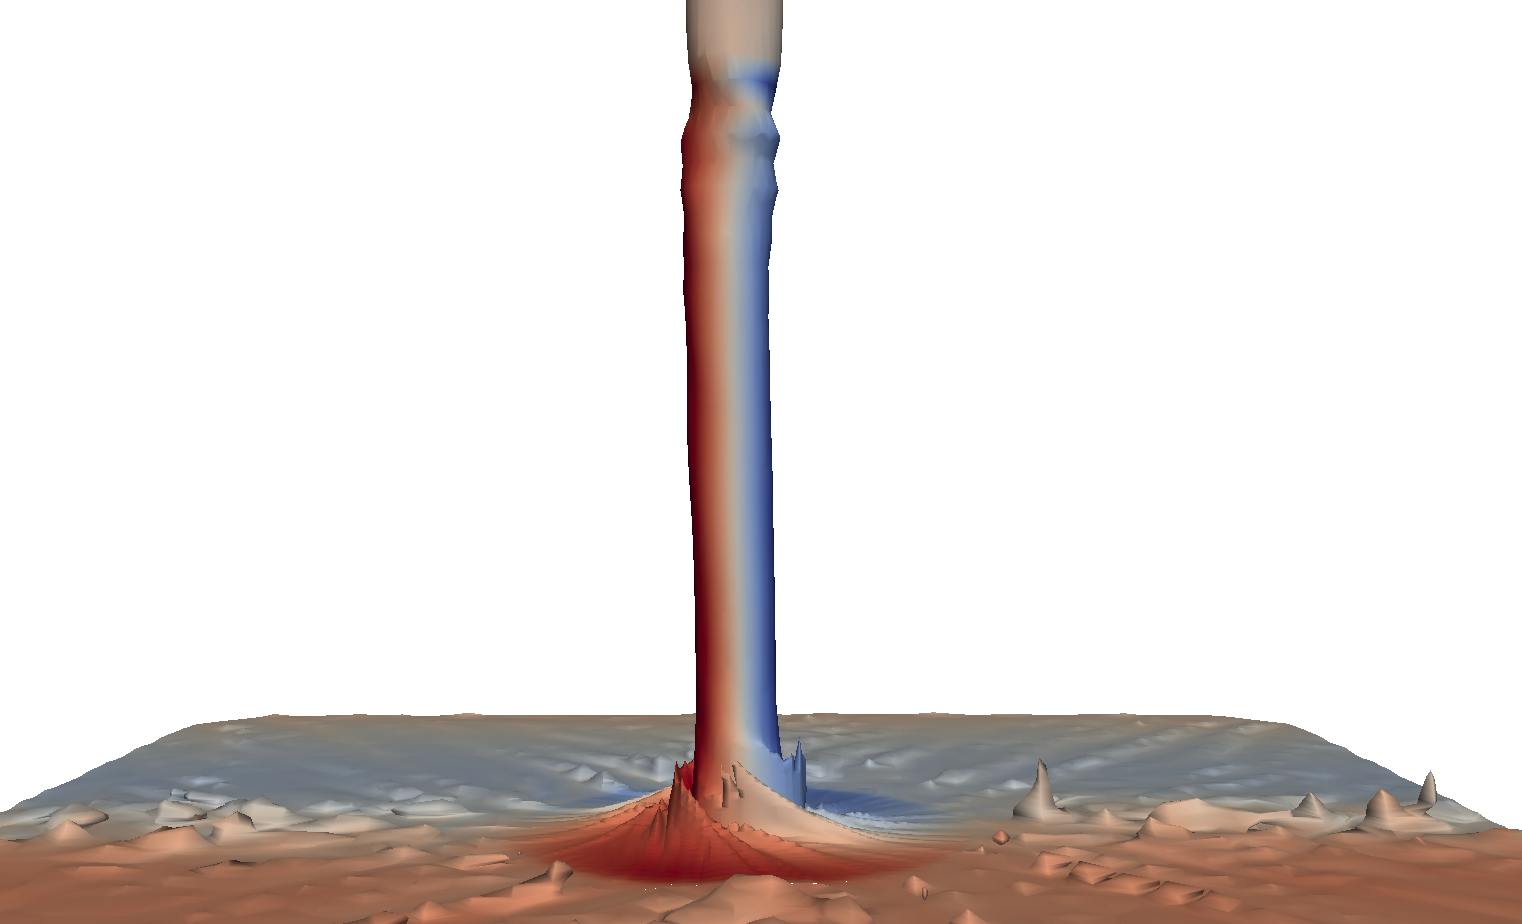
\includegraphics[width=\linewidth]{figs/3m_temp_iso}
  \caption{3m Apparatus}\label{fig:3m_scaling}
\endminipage\hfill
\minipage{0.32\textwidth}%
  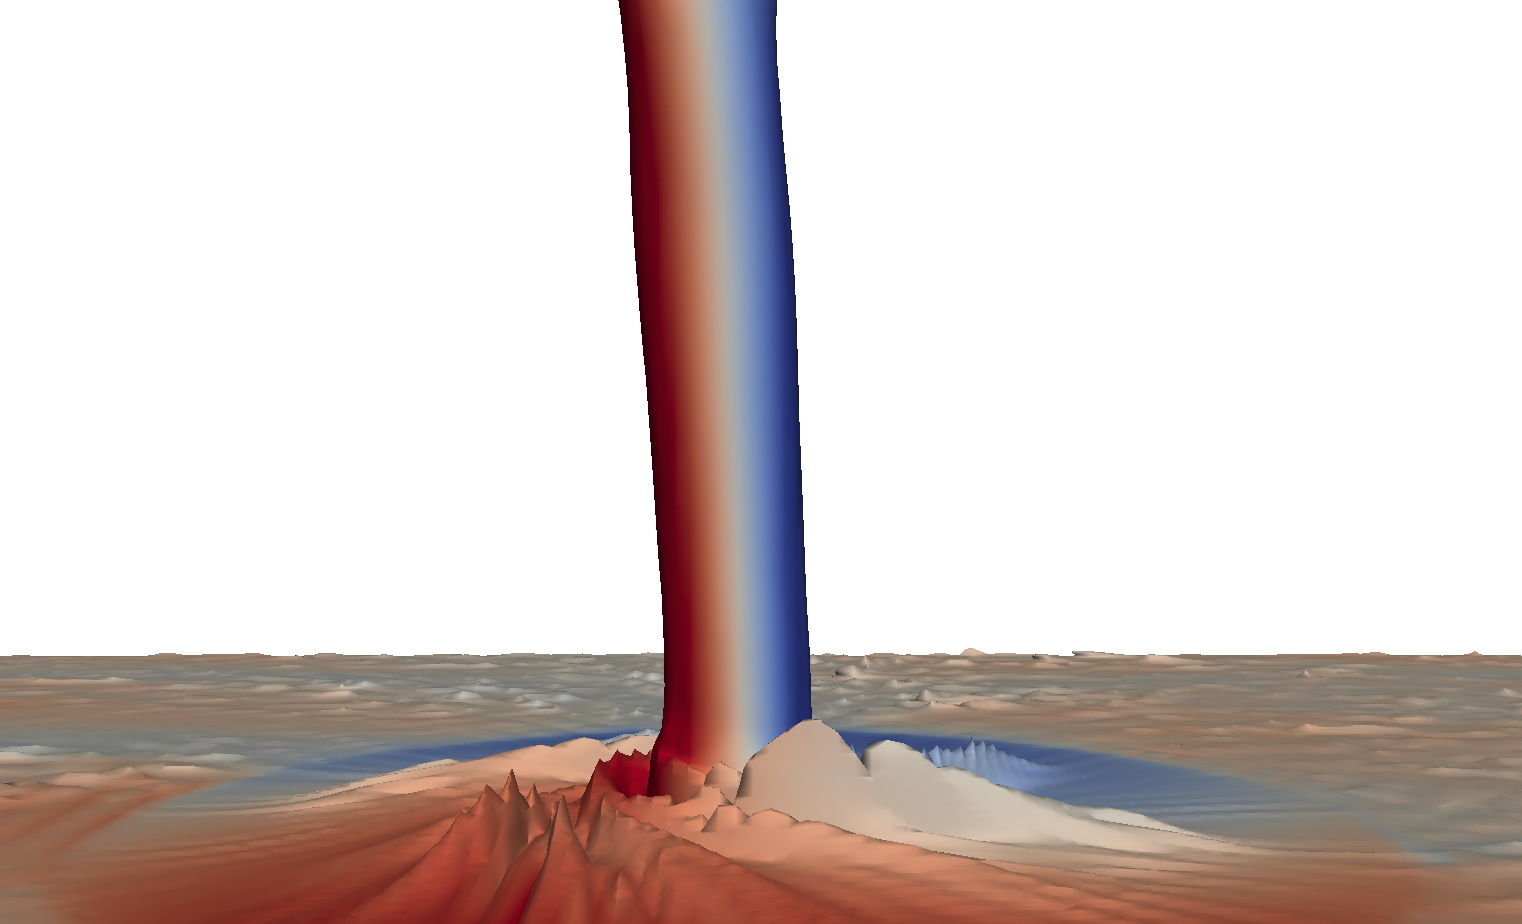
\includegraphics[width=\linewidth]{figs/5m_temp_iso}
  \caption{5m Apparatus}\label{fig:5m_scaling}
\endminipage
\end{figure}


  %% \begin{figure}[!htb]
  %%   \begin{center}
  %%    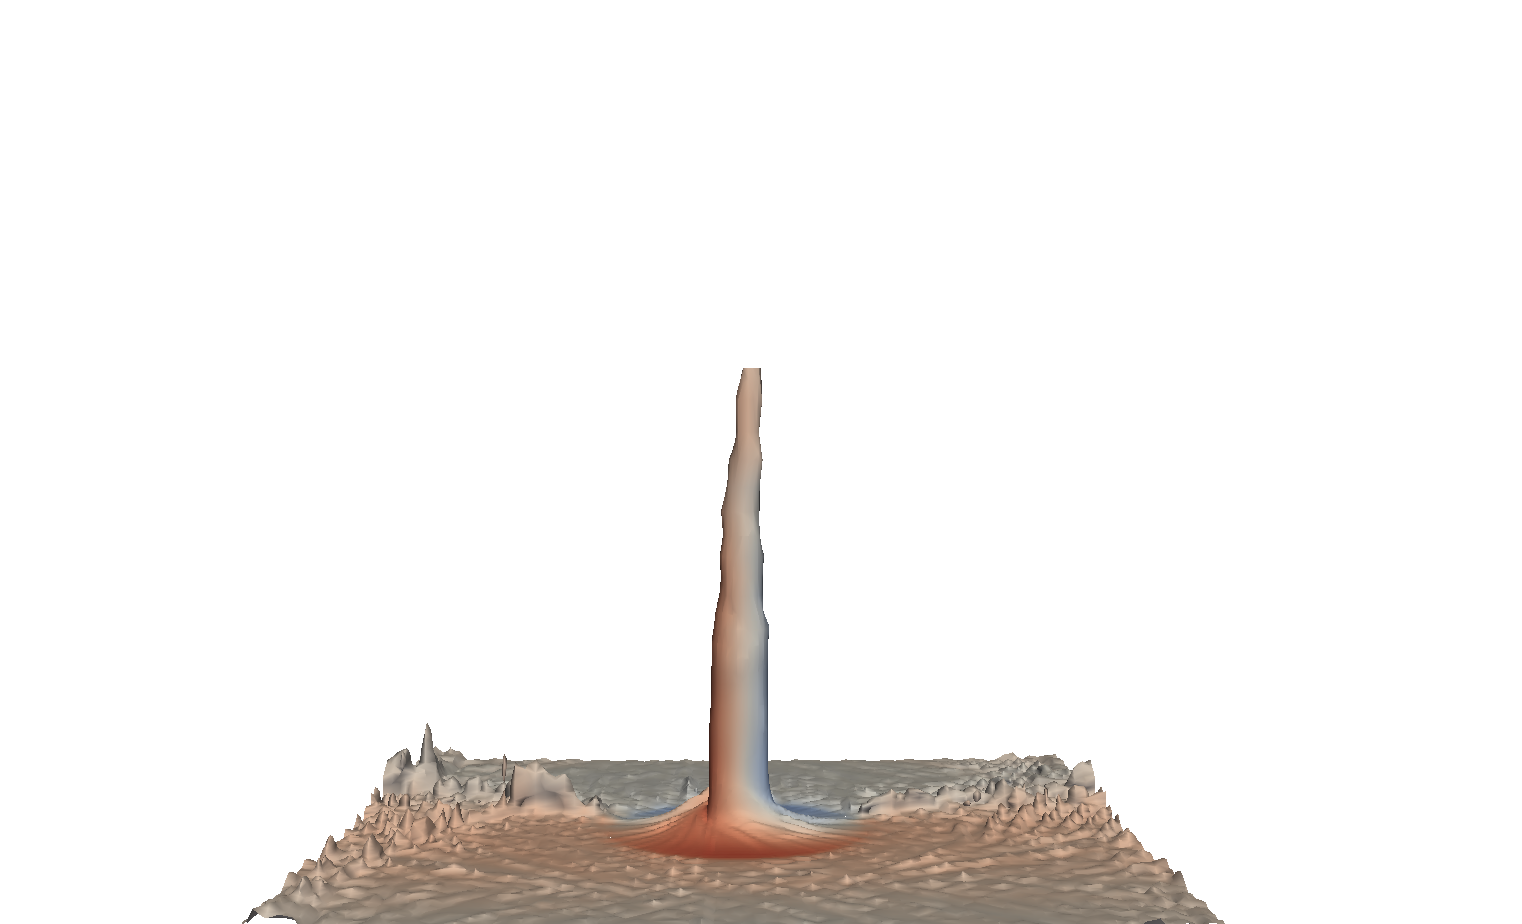
\includegraphics[width = 12 cm]{figs/1m_temp_iso}
  %%    \caption{1m }
  %%    \label{lab}
  %%   \end{center}
  %% \end{figure}


\end{document}
